\documentclass[10pt]{exam}
\usepackage[hon]{template-for-exam}
\usepackage{pgfplots,hyperref}
\pgfplotsset{compat=1.18,
  axis y line = box,
  axis x line = box,
  axis y line shift = 0,
  axis line style = thin,
  xlabel={$t$},
  ylabel={$x(t)$},
  ymin=-9.4,
  ymax=9.4,
  xmin=0,
  xmax=3.5,
  grid=both,
  minor tick num=29,
  xtick = {0,10},
  ytick = {-15,15},
  width=\textwidth,
  height=8cm,
  axis y line = center,
  axis x line = center,
  domain=0:15,
  samples=800,
}

\title{Equations of Motion in SHO's}
\author{Rohrbach}
\date{\today}

\begin{document}
\maketitle

\begin{questions}

\question 
  An object of mass 0.75~kg oscillates according to the equation
  %
  \begin{align*}
    y_1(t)=0.50\cos\left(12.47 \cdot t\right) \, ,
  \end{align*}
  %
  where $x$ is measured in meters and $t$ is measured in seconds.


  \begin{parts}
    \part
      What is the amplitude? \label{amp}
    \part
      What is the frequency? \label{freq}
    \part
      What is the total energy of the system?

    \vs[4]

    \part
      Plot the equation on Desmos (\href{http://www.desmos.com/calculator}{\texttt{www.desmos.com/calculator}}) and explain how it the resulting graph matches your answers for (\ref{amp}) and (\ref{freq}).
      \vs

    \part 
      Where will the mass on the end of the spring be located at $t=1.6$~s?
      \vs

    \part 
      Also plot 
      %
      \begin{align*}
        y_2(t)=0.50 \sin\left(12.47 \cdot t\right) \, .
      \end{align*}
      %
      What's the difference between these two graphs?  See if you can find a phase shift $\phi$ that makes these graphs the same.

      \vs

  \end{parts}


\question
  Now, try plotting $x(t)=A\sin(2\pi f \cdot t + \phi)$ on Desmos. Use the ``slider'' capability of Desmos to investigate how changing $f$ and $A$ changes the graph.


\end{questions}

\pagebreak

\section*{Damped Harmonic Motion}


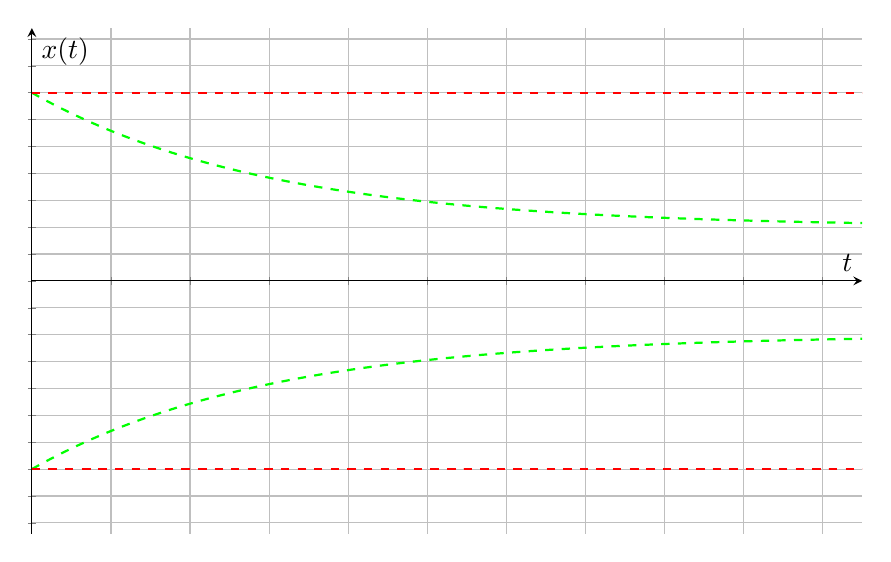
\begin{tikzpicture}
  \begin{axis}
    \addplot[thick,dashed,green,smooth]{5*exp(-x)+2};
    \addplot[thick,dashed,green,smooth]{-5*exp(-x)-2};
    \addplot[thick,dashed,red,smooth]{7};
    \addplot[thick,dashed,red,smooth]{-7};
  \end{axis}
\end{tikzpicture}

\vspace{3em}

\noindent
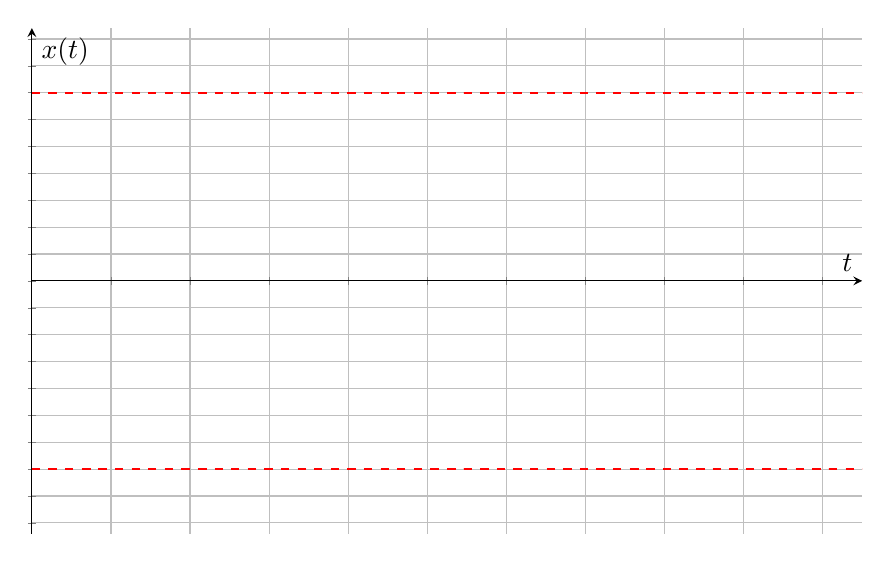
\begin{tikzpicture}
  \begin{axis}
    \addplot[thick,dashed,red,smooth]{7};
    \addplot[thick,dashed,red,smooth]{-7};
  \end{axis}
\end{tikzpicture}


\end{document}